\usetikzlibrary{calc}
\usetikzlibrary{chains, decorations.pathreplacing, positioning}

\definecolor{decoration}{RGB}{0, 122, 195} %CTU blue
\definecolor{heading}{RGB}{0, 122, 195}
\definecolor{headbackgroundgray}{RGB}{199, 219, 241} %light blue
\definecolor{backgroundgray}{RGB}{199, 219, 241} %CTU light blue
\definecolor{headgray}{rgb}{0.50,0.50,0.51}
\definecolor{enumgray}{RGB}{0, 122, 195} %CTU blue

\begin{figure}[!ht]

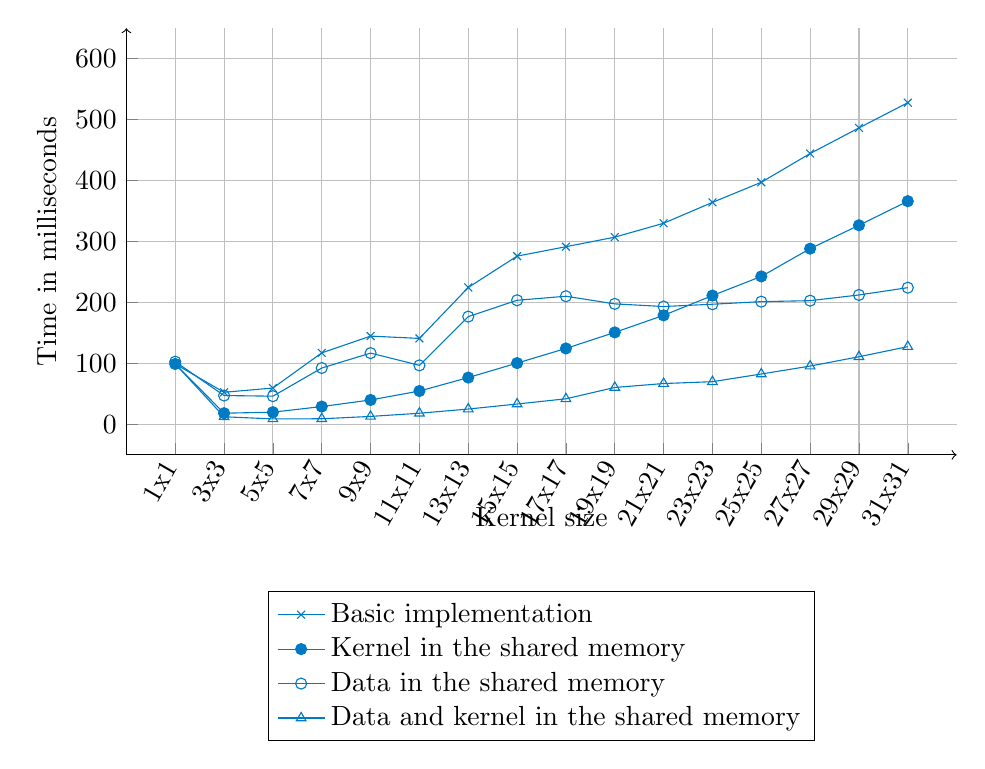
\begin{tikzpicture}
\begin{axis}[
  width=\textwidth,
  height = 7cm,
  axis y line*=left,
  axis x line*=bottom,
  xmin=0,xmax=17,
  ymin=-0.05,ymax=0.65,
  xlabel=Kernel size ,
  axis line style={->},
  grid=both,
  xticklabels={1x1, 3x3, 5x5, 7x7, 9x9, 11x11, 13x13, 15x15, 17x17, 19x19, 21x21, 23x23, 25x25, 27x27, 29x29, 31x31},
  yticklabels={0, 100, 200, 300, 400, 500, 600},
  x label style={at={(axis description cs:0.5,-0.1)},anchor=north},
  xtick={1,...,16},
  ytick={0, 0.1, 0.2, 0.3,  0.4,  0.5, 0.6},
  x tick label style={rotate=60,anchor=east},
  legend style={at={(0.5,-0.32)},anchor=north,legend cell align=left},
  ylabel=Time in milliseconds]

  \addplot[color=enumgray,mark=x] coordinates {
		(1, 0.09905987)
    (2, 0.05264292)
    (3, 0.05966551)
    (4, 0.1173311)
    (5, 0.1448225)
    (6, 0.1410601)
    (7, 0.2246433)
    (8, 0.2760581)
    (9, 0.2915316)
    (10, 0.3071894)
    (11, 0.3300279)
    (12, 0.3642364)
    (13, 0.3972341)
    (14, 0.4444033)
    (15, 0.4864762)
    (16, 0.5278137)
	};

  \addplot[color=enumgray,mark=*] coordinates {
		(1, 0.09908728)
    (2, 0.01832195)
    (3, 0.02002672)
    (4, 0.02923423)
    (5, 0.04007659)
    (6, 0.0547308)
    (7, 0.07679847)
    (8, 0.1005561)
    (9, 0.1245871)
    (10, 0.1509273)
    (11, 0.1788827)
    (12, 0.2113927)
    (13, 0.242748)
    (14, 0.288322)
    (15, 0.3266876)
    (16, 0.3661957)
	};

  \addplot[color=enumgray,mark=o] coordinates {
		(1, 0.1029016)
    (2, 0.0473262)
    (3, 0.0462762)
    (4, 0.09247403)
    (5, 0.1169526)
    (6, 0.0968313)
    (7, 0.17683)
    (8, 0.2036186)
    (9, 0.2102578)
    (10, 0.1976996)
    (11, 0.1933833)
    (12, 0.1971287)
    (13, 0.2013743)
    (14, 0.202982)
    (15, 0.2123374)
    (16, 0.2243093)
	};

  \addplot[color=enumgray,mark=triangle] coordinates {
		(1, 0.09924878)
    (2, 0.01248039)
    (3, 0.008988385)
    (4, 0.009190128)
    (5, 0.013064)
    (6, 0.01828506)
    (7, 0.025166)
    (8, 0.03340602)
    (9, 0.04198433)
    (10, 0.06056602)
    (11, 0.06701268)
    (12, 0.07003736)
    (13, 0.08267156)
    (14, 0.09565835)
    (15, 0.1109782)
    (16, 0.1275336)
	};

  \addlegendentry{Basic implementation}
  \addlegendentry{Kernel in the shared memory}
  \addlegendentry{Data in the shared memory}
  \addlegendentry{Data and kernel in the shared memory}
\end{axis}
\end{tikzpicture}

\caption{The evaluation times of different convolution operator implementations for different kernel sizes on the 8192x8192 domain}
\label{fig:convolve-result}

\end{figure}